\documentclass{standalone}
% \documentclass{article}

\usepackage{tikz}

\begin{document}

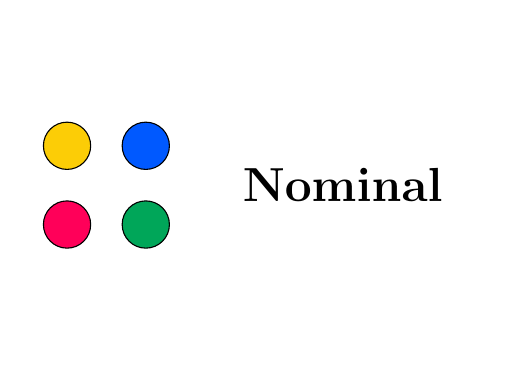
\begin{tikzpicture}
\draw[draw=none, fill=none] (0, -1) rectangle (6, 3);
\node at (4, 1) {\LARGE{\textbf{Nominal}}};
\draw[draw=black, fill=red!65!magenta] (0.5, 0.5) circle (0.3);
\draw[draw=black, fill=yellow!65!orange] (0.5, 1.5) circle (0.3);
\draw[draw=black, fill=green!65!blue] (1.5, 0.5) circle (0.3);
\draw[draw=black, fill=blue!65!cyan] (1.5, 1.5) circle (0.3);
\end{tikzpicture}

\end{document}
